%%%%%%%%%%%%%%%%%%%%%%%%%%%%%%%%%%%%%%%%%
% Beamer Presentation
% LaTeX Template
% Version 1.0 (10/11/12)
%
% This template has been downloaded from:
% http://www.LaTeXTemplates.com
%
% License:
% CC BY-NC-SA 3.0 (http://creativecommons.org/licenses/by-nc-sa/3.0/)
%
%%%%%%%%%%%%%%%%%%%%%%%%%%%%%%%%%%%%%%%%%

%----------------------------------------------------------------------------------------
%	PACKAGES AND THEMES
%----------------------------------------------------------------------------------------

\documentclass{beamer}

\mode<presentation> {

% The Beamer class comes with a number of default slide themes
% which change the colors and layouts of slides. Below this is a list
% of all the themes, uncomment each in turn to see what they look like.

%\usetheme{default}
%\usetheme{AnnArbor}
%\usetheme{Antibes}
%\usetheme{Bergen}
%\usetheme{Berkeley}
%\usetheme{Berlin}
%\usetheme{Boadilla}
%\usetheme{CambridgeUS}
%\usetheme{Copenhagen}
%\usetheme{Darmstadt}
%\usetheme{Dresden}
%\usetheme{Frankfurt}
%\usetheme{Goettingen}
%\usetheme{Hannover}
%\usetheme{Ilmenau}
%\usetheme{JuanLesPins}
%\usetheme{Luebeck}
%\usetheme{Madrid}
%\usetheme{Malmoe}
%\usetheme{Marburg}
%\usetheme{Montpellier}
%\usetheme{PaloAlto}
\usetheme{Pittsburgh}
%\usetheme{Rochester}
%\usetheme{Singapore}
%\usetheme{Szeged}
%\usetheme{Warsaw}

% As well as themes, the Beamer class has a number of color themes
% for any slide theme. Uncomment each of these in turn to see how it
% changes the colors of your current slide theme.

%\usecolortheme{albatross}
\usecolortheme{beaver}
%\usecolortheme{beetle}
%\usecolortheme{crane}
%\usecolortheme{dolphin}
%\usecolortheme{dove}
%\usecolortheme{fly}
%\usecolortheme{lily}
%\usecolortheme{orchid}
%\usecolortheme{rose}
%\usecolortheme{seagull}
%\usecolortheme{seahorse}
%\usecolortheme{whale}
%\usecolortheme{wolverine}

%\setbeamertemplate{footline} % To remove the footer line in all slides uncomment this line
%\setbeamertemplate{footline}[page number] % To replace the footer line in all slides with a simple slide count uncomment this line

%\setbeamertemplate{navigation symbols}{} % To remove the navigation symbols from the bottom of all slides uncomment this line
}
\usepackage{graphicx} % Allows including images
\usepackage{booktabs} % Allows the use of \toprule, \midrule and \bottomrule in tables

\usepackage{fontspec}
\setsansfont{Calibri}[
    Path=Font/,
    Scale=0.9,
    Extension = .ttf,
    UprightFont=*-Regular,
    BoldFont=*-Bold,
    ItalicFont=*-Italic,
    BoldItalicFont=*-BoldItalic
    ]
\usepackage{unicode-math}
\setmathfont{Libertinus Math}% 使用默认的数学字体或你偏好的数学字体 Latin Modern Math/Libertinus Math
% \setmathfont[version=bold]{Latin Modern Math}

% ---- 中文支持（xeCJK）：用 XeLaTeX 编译 ----
\usepackage{xeCJK}
\setCJKmainfont{Songti SC}
\setCJKsansfont{Heiti SC}
\setCJKmonofont{Heiti SC}
\xeCJKsetup{AutoFakeBold=true, AutoFakeSlant=true}

\usepackage{tikz}
\usetikzlibrary{positioning}
\usetikzlibrary{calc}
\usepackage{ragged2e}
\justifying\let\raggedright\justifying %两端对齐
%----------------------------------------------------------------------------------------
%	TITLE PAGE
%----------------------------------------------------------------------------------------

\title[资产定价]{\textbf{资产定价}} % The short title appears at the bottom of every slide, the full title is only on the title page

\subtitle{6. 基于生产的资产定价}

\author[Cheng Hang]{Cheng Hang} % Your name
\institute[DUFE] % Your institution as it will appear on the bottom of every slide, may be shorthand to save space
{金融科技学院 \\
东北财经大学 \\ % Your institution for the title page
\medskip
\textbf{chenghangch@qq.com}% Your email address
}
\date{\today} % Date, can be changed to a custom date

	\AtBeginSection[]
{
	\begin{frame}[allowframebreaks]{目录}
		\small
		\tableofcontents[sectionstyle=show/shaded,subsectionstyle=show/shaded/hide] %这几个参数我也不知道该如何准确地解释，反正它们最终的效果是突出显示当前章节，而其它章节都进行了淡化处理
		\addtocounter{framenumber}{-1}  %目录页不计算页码
	\end{frame}
}

%----------------------------------------------------------------------------------------
%	Begin
%----------------------------------------------------------------------------------------

\begin{document}

\begin{frame}
\titlepage % Print the title page as the first slide
\end{frame}

%\begin{frame}
%\frametitle{Overview} % Table of contents slide, comment this block out to remove it
%\tableofcontents % Throughout your presentation, if you choose to use \section{} and \subsection{} commands, these will automatically be printed on this slide as an overview of your presentation
%\end{frame}

%--------------------------------------
%	PRESENTATION SLIDES
%--------------------------------------

\begin{frame}{路线图与一句话主线}
	本讲是三讲弧线中的\textbf{第二幕}。
	\vspace{4pt}
	\begin{center}
		\small
		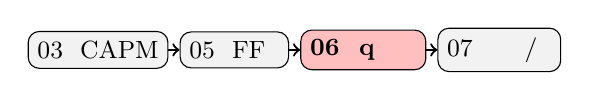
\begin{tikzpicture}[node distance=4pt, every node/.style={font=\small}]
			\node[draw,rounded corners,fill=gray!10] (a) {03~~CAPM};
			\node[draw,rounded corners,fill=gray!10,right=of a] (b) {05~~FF因子};
			\node[draw,rounded corners,fill=red!25,right=of b] (c) {\textbf{06~~q因子（本讲）}};
			\node[draw,rounded corners,fill=gray!10,right=of c] (d) {07~~因子动物园/战争};
			\draw[->,thick] (a) -- (b);
			\draw[->,thick] (b) -- (c);
			\draw[->,thick] (c) -- (d);
		\end{tikzpicture}
	\end{center}
	\textbf{05 讲的终点。} FF3 无法为四个重要异象定价——\textbf{动量、盈利、投资、特质波动率（IVOL）}。两条修补路线：继续添加经验因子（FF5/FF6），或从结构模型中\textit{推导}出因子。\textbf{本讲走结构化路线。}
	\begin{block}{一句话概括整讲}
		\[
			\underbrace{\mathrm{E}_t[1+R^S_{i,t+1}]}_{\text{预期股票毛收益率}}
			\;=\; \frac{\;\mathrm{E}_t[\text{盈利能力}_{i,t+1}]\;}{\;\underbrace{1+a\,(I_{it}/K_{it})}_{\text{投资的边际成本}}\;}
		\]
		下面的全部内容都将\textbf{从企业最优化出发推导}出该式，并解读其横截面含义。
	\end{block}
	\href{https://theinvestmentcapm.com/index.html}{\textcolor{blue}{张橹的网站：The Investment CAPM}}
\end{frame}

\begin{frame}[allowframebreaks]{两种范式：需求侧 vs.\ 供给侧}
	\small
	\begin{tabular}{@{}p{0.46\linewidth}p{0.46\linewidth}@{}}
		\toprule
		\textbf{需求侧（基于消费）} & \textbf{供给侧（基于生产）} \\
		\midrule
		投资者欧拉方程：$1=\mathrm{E}_t[M_{t+1}(1+R_{t+1})]$。 & 企业投资欧拉方程：$1=\mathrm{E}_t[M_{t+1}(1+R^I_{t+1})]$。 \\
		\addlinespace
		定价核来自消费的边际效用／模拟组合。 & 定价核由投资的边际成本与边际收益约束。 \\
		\addlinespace
		因子\textit{事后}由异象组合构造。 & 因子由企业一阶条件\textit{事前}决定。 \\
		\addlinespace
		CCAPM、ICAPM、FF3/5/6。 & \href{https://doi.org/10.1111/j.1540-6261.1991.tb03750.x}{\textcolor{blue}{Cochrane (1991)}}、\href{https://doi.org/10.1086/649760}{\textcolor{blue}{LWZ (2009)}}、\href{https://doi.org/10.1093/rfs/hhu068}{\textcolor{blue}{HXZ (2015)}} $q$、HMXZ (2021) $q^5$。 \\
		\bottomrule
	\end{tabular}
	\break
	\begin{block}{我们将要证明的命题}
		\[
			\underbrace{1+R^S_{t+1}}_{\text{金融收益率（股票市场）}}=\underbrace{1+R^I_{t+1}}_{\text{投资收益率（实体经济）}}
		\]
		在均衡中，对企业的金融索取权的收益率\textit{必然}等于其边际实物投资的收益率。因此，各企业在 $I/K$ 与盈利能力上的差异\textit{必然}体现为预期股票收益率的差异。
	\end{block}
\end{frame}

\begin{frame}
	\begin{figure}
		\centering
		
\includegraphics[width=1\linewidth]{Files/qfactor.jpg}
	\end{figure}
\end{frame}

\begin{frame}{基于生产的框架：四个要件}
	\begin{enumerate}
		\item \textbf{技术：}柯布--道格拉斯 $X_t=Z_tK_t^\alpha L_t^{1-\alpha}$（规模报酬不变）。
		\item \textbf{调整成本：}凸的 $\Phi_t=\phi(I_t/K_t)K_t$，其中 $\phi'>0,\ \phi''\ge 0$。
		\item \textbf{最优化：}企业最大化 $V_t=\max \mathrm{E}_t\sum_{s\ge0}M_{t,t+s}D_{t+s}$。
		\item \textbf{结论：}投资 $I/K$ 与盈利能力 $Y/K$ 决定预期收益率。
	\end{enumerate}
	\vspace{4pt}
	阐述遵循 \textcolor{blue}{\href{https://doi.org/10.1146/annurev-financial-110311-101731}{Kogan and Papanikolaou (2012)}}；结构估计遵循 \textcolor{blue}{\href{https://doi.org/10.1086/649760}{Liu, Whited, and Zhang (2009)}}。
	\begin{block}{如何阅读这些数学}
		我们先\textbf{搭建机器}（技术 $\to$ 一阶条件 $\to$ 投资收益率），再\textbf{将其转化为可检验的收益率}，最后给出\textbf{张橹的横截面发现}与 $q$ 因子模型。
	\end{block}
\end{frame}

\section{构件：技术与最优化}

\begin{frame}{技术与最优劳动选择}
	\textbf{柯布--道格拉斯生产函数（规模报酬不变）：}
	\begin{equation}\label{equ:production}
		X_t = Z_t K_t^\alpha L_t^{1-\alpha},\qquad \alpha\in(0,1).
	\end{equation}
	\textbf{劳动为静态选择}（将 $K_t,\omega_t$ 视为给定），故其一阶条件令劳动的边际产出等于工资：
	\begin{equation*}
		\max_{L_t}\{X_t-\omega_t L_t\}\ \Rightarrow\ \frac{\partial X_t}{\partial L_t}=(1-\alpha)Z_tK_t^\alpha L_t^{-\alpha}=\omega_t.
	\end{equation*}
	\textbf{求解劳动需求：}
	\begin{equation}\label{equ:optimal labor supply}
		L_t^*=\left(\frac{(1-\alpha)Z_t}{\omega_t}\right)^{1/\alpha}K_t.
	\end{equation}
	\vspace{2pt}
	\textit{为何这样做。}将 $L_t^*$ 代回，可把双投入的技术化为\textbf{单状态}（仅资本）问题，并使利润与资本的边际产出成正比——这正是为收益率定价的对象。
\end{frame}

\begin{frame}{盈利能力等于产出的资本份额}
	\textbf{最优劳动下的产出}——将（\ref{equ:optimal labor supply}）代入（\ref{equ:production}）：
	\begin{equation*}
		\begin{aligned}
			Y_t &= Z_t K_t^\alpha (L_t^*)^{1-\alpha}
			= Z_t K_t^\alpha\left[\left(\tfrac{(1-\alpha)Z_t}{\omega_t}\right)^{1/\alpha}K_t\right]^{1-\alpha}\\
			&= Z_t^{1/\alpha}\left(\frac{1-\alpha}{\omega_t}\right)^{(1-\alpha)/\alpha}K_t
			\;\Rightarrow\; \frac{Y_t}{K_t}=Z_t^{1/\alpha}\left(\frac{1-\alpha}{\omega_t}\right)^{(1-\alpha)/\alpha}.
		\end{aligned}
	\end{equation*}
	\textbf{支付劳动后的毛利润：}
	\begin{equation}\label{equ: gross profit}
		\Pi_t=Y_t-\omega_t L_t^* = Y_t-(1-\alpha)\underbrace{Z_t^{1/\alpha}\!\left(\tfrac{1-\alpha}{\omega_t}\right)^{(1-\alpha)/\alpha}K_t}_{=\,Y_t}=\alpha Y_t.
	\end{equation}
	\begin{block}{携带至后文的两个事实}
		(i) 利润 $\Pi_t=\alpha Y_t$——产出中资本的份额（美国数据中 $\alpha\approx 1/3$）。 \\
		(ii) 产出关于 $K_t$ 线性，故\textbf{资本的边际产出等于平均盈利能力}：$\partial Y_t/\partial K_t = Y_t/K_t$。这一“盈利能力”位于下文每个收益率公式的分子。
	\end{block}
\end{frame}

\section{含调整成本的投资决策}

\begin{frame}{资本积累与调整成本}
	\textbf{资本的运动方程：}
	\begin{equation}\label{equ:capital accumulation}
		K_{t+1}=I_t+(1-\delta)K_t,\qquad \delta\in(0,1).
	\end{equation}
	\textbf{总投资成本}（关于 $(I_t,K_t)$ 规模报酬不变）：
	\begin{equation}\label{equ:investment cost}
		\Phi_t=\phi\!\left(\frac{I_t}{K_t}\right)K_t,\qquad \phi'>0,\ \phi''\ge 0,\ \phi(0)=0.
	\end{equation}
	\textbf{为何调整成本不可或缺。}
	\begin{itemize}
		\item 没有它们（Hayashi：$\phi(I/K)=I/K$，故 $\Phi_t=I_t$），资本会瞬间跳至目标值，投资对 $q$ 的弹性无穷大——与事实不符。
		\item 凸成本（安装、扰动、再培训、转售折价）使投资\textbf{迟缓且前瞻}，并赋予 $\phi'(\cdot)$ 非平凡的斜率——这是收益率变动的引擎。
	\end{itemize}
\end{frame}

\begin{frame}{股利与公司价值}
	\textbf{股利（流向股东的现金流）：}
	\begin{equation}\label{equ:dividend}
		D_t=\Pi_t-\Phi_t=\alpha Y_t-\phi\!\left(\frac{I_t}{K_t}\right)K_t.
	\end{equation}
	\textbf{公司价值（股利的现值）：}
	\begin{equation}\label{equ:firm value}
		V_t=\mathrm{E}_t\sum_{s=0}^{\infty}M_{t,t+s}D_{t+s},
	\end{equation}
	其中 $M_{t,t+s}$ 是从 $t$ 到 $t+s$ 的随机折现因子。
	\begin{itemize}
		\item 经理选择 $I_t$ 以最大化 $V_t$。
		\item 当期投资通过资本积累（\ref{equ:capital accumulation}）影响\textit{所有}未来现金流——这是动态权衡的来源。
	\end{itemize}
\end{frame}

\section{企业的最优化问题}

\begin{frame}{动态规划表述}
    \textbf{贝尔曼方程：}
    \begin{equation}\label{equ:bellman}
        V_t = \max_{I_t} \left\{ D_t + \mathrm{E}_t\left[M_{t+1} V_{t+1}\right] \right\}
    \end{equation}

    \textbf{解读：}
    \begin{itemize}
        \item 今日价值 = 今日股利 + 折现的预期未来价值
        \item 选择变量：投资 $I_t$
        \item 权衡：
        \begin{itemize}
            \item 更高的 $I_t$ $\rightarrow$ 今日更低的 $D_t$（需要花钱）
            \item 但更高的 $K_{t+1}$ $\rightarrow$ 明日更高的 $V_{t+1}$（更多产出）
        \end{itemize}
    \end{itemize}


    \textbf{一阶条件：}
    \begin{equation}\label{equ:foc}
        \frac{\partial D_t}{\partial I_t} + \mathrm{E}_t\left[M_{t+1} \frac{\partial V_{t+1}}{\partial I_t}\right] = 0
    \end{equation}

    利用 $\frac{\partial D_t}{\partial I_t} = -\phi'\left(\frac{I_t}{K_t}\right)$ 与 $\frac{\partial V_{t+1}}{\partial I_t} = \frac{\partial V_{t+1}}{\partial K_{t+1}}$：
    \begin{equation}\label{equ:marginal}
        \phi'\left(\frac{I_t}{K_t}\right) = \mathrm{E}_t\left[M_{t+1} \frac{\partial V_{t+1}}{\partial K_{t+1}}\right]
    \end{equation}
\end{frame}

\begin{frame}[allowframebreaks]{解读一阶条件}
    \begin{equation*}
        \underbrace{\phi'\left(\frac{I_t}{K_t}\right)}_{\text{投资的边际成本}} = \underbrace{\mathrm{E}_t\left[M_{t+1} \frac{\partial V_{t+1}}{\partial K_{t+1}}\right]}_{\text{折现的预期边际收益}}
    \end{equation*}


    \textbf{左端（边际成本）：}
    \begin{itemize}
        \item 今日多投资一单位的成本
        \item 包含购置价格 + 调整成本
        \item 减少当期股利
    \end{itemize}


    \textbf{右端（边际收益）：}
    \begin{itemize}
        \item 明日多拥有一单位资本的价值
        \item 由 SDF $M_{t+1}$ 折现（针对风险与时间偏好调整）
        \item 增加未来产出与利润
    \end{itemize}


    \textbf{均衡：}
    \begin{itemize}
        \item 投资直至边际成本 = 预期边际收益
        \item 若 $\phi' < \mathrm{E}[M V']$：增加投资（收益超过成本）
        \item 若 $\phi' > \mathrm{E}[M V']$：减少投资（成本超过收益）
    \end{itemize}
\end{frame}

\begin{frame}{包络定理}
    \textbf{目标：}推导资本的边际价值 $\frac{\partial V_{t+1}}{\partial K_{t+1}}$。

    由包络定理，在固定最优投资选择的前提下，对状态变量微分贝尔曼方程；再推进一期：
    \begin{equation}\label{equ:envelope}
        \frac{\partial V_{t+1}}{\partial K_{t+1}} = \underbrace{\frac{\partial D_{t+1}}{\partial K_{t+1}}}_{\text{步骤 1：当期股利}} + \underbrace{\mathrm{E}_{t+1}\left[M_{t+2} \frac{\partial V_{t+2}}{\partial K_{t+1}}\right]}_{\text{步骤 2--3：延续价值}}
    \end{equation}

    \textbf{步骤 1：对股利微分} $D_{t+1} = \alpha Y_{t+1} - \Phi_{t+1}$，其中 $\Phi_{t+1} \equiv \phi\!\left(\frac{I_{t+1}}{K_{t+1}}\right) K_{t+1}$：
    \begin{equation*}
        \frac{\partial D_{t+1}}{\partial K_{t+1}} = \alpha \frac{\partial Y_{t+1}}{\partial K_{t+1}} - \frac{\partial \Phi_{t+1}}{\partial K_{t+1}}
    \end{equation*}
\end{frame}

\begin{frame}{包络定理：成本项}
    \textbf{步骤 1（续）：}对投资成本项微分。

    对 $\Phi_{t+1} = \phi(I_{t+1}/K_{t+1}) \cdot K_{t+1}$ 应用\textbf{乘积法则}：
    \begin{equation*}
        \begin{aligned}
            \frac{\partial \Phi_{t+1}}{\partial K_{t+1}} &= \underbrace{\phi'\!\left(\tfrac{I_{t+1}}{K_{t+1}}\right) \cdot \left(-\tfrac{I_{t+1}}{K_{t+1}^2}\right) \cdot K_{t+1}}_{\text{对 } \phi(I/K) \text{ 用链式法则}} + \underbrace{\phi\!\left(\tfrac{I_{t+1}}{K_{t+1}}\right) \cdot 1}_{\text{对 } K \text{ 求导}} \\
            &= \phi\!\left(\tfrac{I_{t+1}}{K_{t+1}}\right) - \phi'\!\left(\tfrac{I_{t+1}}{K_{t+1}}\right) \tfrac{I_{t+1}}{K_{t+1}}
        \end{aligned}
    \end{equation*}

    \vspace{4pt}
    \textbf{为何重要：}在固定投资的情况下，更大的资本基数会降低投资率 $I/K$，从而改变调整成本。
\end{frame}

\begin{frame}{包络定理（续）}
    \textbf{步骤 2：对未来价值项使用链式法则}
    \begin{equation*}
        \frac{\partial V_{t+2}}{\partial K_{t+1}} = \frac{\partial V_{t+2}}{\partial K_{t+2}} \cdot \frac{\partial K_{t+2}}{\partial K_{t+1}} = \frac{\partial V_{t+2}}{\partial K_{t+2}} (1-\delta)
    \end{equation*}

    因为 $K_{t+2} = I_{t+1} + (1-\delta)K_{t+1}$，且包络步骤固定 $I_{t+1}$（只有未折旧的资本起作用）


    \textbf{步骤 3：将一阶条件（\ref{equ:marginal}）向前推进一期}
    \begin{equation*}
        \mathrm{E}_{t+1}\left[M_{t+2} \frac{\partial V_{t+2}}{\partial K_{t+2}}\right] = \phi'\left(\frac{I_{t+1}}{K_{t+1}}\right)
    \end{equation*}


    \textbf{最终结果（包络定理）：}
    \begin{equation}\label{equ:envelope theorem}
        \boxed{
        \frac{\partial V_{t+1}}{\partial K_{t+1}} = \alpha \frac{\partial Y_{t+1}}{\partial K_{t+1}} - \frac{\partial \Phi_{t+1}}{\partial K_{t+1}} + (1-\delta) \phi'\left(\frac{I_{t+1}}{K_{t+1}}\right)
        }
    \end{equation}
\end{frame}

\begin{frame}{包络定理的经济学解读}
    \begin{equation*}
        \frac{\partial V_{t+1}}{\partial K_{t+1}} = \underbrace{\alpha \frac{\partial Y_{t+1}}{\partial K_{t+1}}}_{\text{（1）利润贡献}} - \underbrace{\frac{\partial \Phi_{t+1}}{\partial K_{t+1}}}_{\text{（2）成本效应}} + \underbrace{(1-\delta) \phi'\left(\frac{I_{t+1}}{K_{t+1}}\right)}_{\text{（3）残值}}
    \end{equation*}


    \textbf{三个组成部分：}
    \begin{enumerate}
        \item \textbf{边际利润：}额外产出 $\times$ 利润份额 $\alpha$
        \begin{itemize}
            \item 更多资本 $\rightarrow$ 更多产出 $\rightarrow$ 更多利润
        \end{itemize}

        \item \textbf{成本下降：}更低的平均调整成本
        \begin{itemize}
            \item 更大的资本基数 $\rightarrow$ 同等投资占比更小
            \item 回顾 $\Phi = \phi(I/K) \cdot K$，故当 $I > 0$ 时 $\partial \Phi/\partial K < 0$
        \end{itemize}

        \item \textbf{延续价值：}未折旧资本结转至下期
        \begin{itemize}
            \item 比例 $(1-\delta)$ 存续至下一期
            \item 价值为其安装的边际成本 $\phi'$
        \end{itemize}
    \end{enumerate}

    \vspace{0.2cm}
    \textit{资本的边际价值等于其即时利润贡献与延续价值之和}
\end{frame}

\section{规模报酬不变：托宾 Q}

\begin{frame}{Hayashi（1982）的关键结论}
    \textbf{假设：规模报酬不变（CRS）}
    \begin{itemize}
        \item 生产：$X_t = Z_t K_t^\alpha L_t^{1-\alpha}$ 满足 CRS
        \item 调整成本：$\Phi_t = \phi(I_t/K_t) K_t$ 关于 $(I_t, K_t)$ 满足 CRS
    \end{itemize}


    \textbf{Hayashi 定理：}

    在 CRS 下，边际 $q$ 等于平均 $q$：
    \begin{equation}\label{equ:hayashi}
        \boxed{
        \frac{\partial V_t}{\partial K_t} = \frac{V_t}{K_t}
        }
    \end{equation}


    \textbf{直觉：}
    \begin{itemize}
        \item CRS $\rightarrow$ 所有投入翻倍则产出与价值翻倍
        \item 边际产出与平均产出相等
        \item 公司价值 = 资本的边际价值 $\times$ 资本数量
        \item 关键简化：无需估计边际 $q$，直接用 $V/K$
    \end{itemize}
\end{frame}

\begin{frame}{推导托宾 Q 方程}
    \textbf{从一阶条件（\ref{equ:marginal}）出发：}
    \begin{equation*}
        \phi'\left(\frac{I_t}{K_t}\right) = \mathrm{E}_t\left[M_{t+1} \frac{\partial V_{t+1}}{\partial K_{t+1}}\right]
    \end{equation*}

    \textbf{应用 Hayashi 结论（\ref{equ:hayashi}）：}
    \begin{equation*}
        \phi'\left(\frac{I_t}{K_t}\right) = \mathrm{E}_t\left[M_{t+1} \frac{V_{t+1}}{K_{t+1}}\right]
    \end{equation*}

    \textbf{使用贝尔曼方程：$V_t = D_t + \mathrm{E}_t[M_{t+1} V_{t+1}]$}

    由于 $K_{t+1}$ 在 $t$ 时已知：
    \begin{equation*}
        \phi'\left(\frac{I_t}{K_t}\right) = \frac{\mathrm{E}_t[M_{t+1} V_{t+1}]}{K_{t+1}} = \frac{V_t - D_t}{K_{t+1}}
    \end{equation*}

    \textbf{最终形式（托宾 Q）：}
    \begin{equation}\label{equ:tobins q}
        \boxed{
        \phi'\left(\frac{I_t}{K_t}\right) = \frac{V_t - D_t}{K_{t+1}} = \frac{D_t}{K_{t+1}} \cdot \frac{V_t - D_t}{D_t}
        }
    \end{equation}
\end{frame}

\begin{frame}{拆解托宾 Q}
	\begin{equation*}
		\phi'\!\left(\frac{I_t}{K_t}\right)=\underbrace{\frac{D_t}{K_{t+1}}}_{\text{当期盈利能力}}\times\underbrace{\frac{V_t-D_t}{D_t}}_{\text{价格--股利比}}
	\end{equation*}
	\textbf{解读该恒等式。}
	\begin{itemize}
		\item \textbf{左端}——今日投资的边际成本；由凸性，随 $I_t/K_t$ 上升。
		\item \textbf{右端第一项} $D_t/K_{t+1}$——已安装资本\textit{当下}的盈利程度。
		\item \textbf{右端第二项} $(V_t-D_t)/D_t$——市场为成长机会定的价。
	\end{itemize}
	\vspace{2pt}
	\textbf{经济含义（横截面的种子）。}
	\begin{itemize}
		\item 高 $I/K \Rightarrow$ 右端高 $\Rightarrow$ \textit{要么}当期盈利能力高，\textit{要么}估值丰厚（预期增长强劲），或二者兼有。
		\item 因此\textbf{投资行为揭示}了关于盈利能力与折现率的信息：我们可从可观测的投资中读出预期收益率。下一节将其精确化。
	\end{itemize}
\end{frame}

\section{Cochrane 的投资收益率：通往金融收益率的桥梁}

\begin{frame}{为何要单独定义“投资收益率”？}
    \textbf{回顾：}托宾 Q（\ref{equ:tobins q}）把投资的\textit{水平}与股价的\textit{水平}联系起来。
    \vspace{0.2cm}
    \textbf{水平对水平检验的两个现实问题：}
    \begin{itemize}
        \item 平均 $q = V/K$ 被无形/边际内资产、资本存量的测量误差以及商誉所污染。
        \item $V/K$ 的横截面离散度极大 $\Rightarrow$ 需要不合理地陡峭的 $\phi'(\cdot)$ 才能拟合（\href{https://doi.org/10.1016/0165-1889(93)90022-K}{\textcolor{blue}{Chirinko, 1993}}）。
    \end{itemize}

    \vspace{0.2cm}
    \textbf{\href{https://doi.org/10.1111/j.1540-6261.1991.tb03750.x}{\textcolor{blue}{Cochrane（1991）}}、\href{https://doi.org/10.1086/262034}{\textcolor{blue}{Cochrane（1996）}}：}对水平对水平的关系跨时间／企业作差分。
    \begin{itemize}
        \item 把 $q$ 理论转化为关于\textbf{收益率}而非\textbf{价格}的陈述。
        \item 收益率随时间（高频）与企业（横截面）变化，可吸收固定的测量偏差。
        \item 投资收益率可由会计数据观测：$Y/K$、$I/K$、$\delta$。
    \end{itemize}
\end{frame}

\begin{frame}{定义投资收益率}
    \textbf{步骤 1：整理托宾 Q（$V_t = D_t + \mathrm{E}_t[M_{t+1}V_{t+1}]$）与 Hayashi（\ref{equ:hayashi}）：}
    \begin{equation*}
        \phi'\left(\frac{I_t}{K_t}\right) = \mathrm{E}_t\left[M_{t+1} \frac{\partial V_{t+1}}{\partial K_{t+1}}\right]
    \end{equation*}

    \textbf{步骤 2：定义毛投资收益率}
    \begin{equation}\label{equ:investment return def}
        \boxed{
        1 + R^I_{t+1} \equiv \frac{\partial V_{t+1}/\partial K_{t+1}}{\phi'(I_t/K_t)} = \frac{\text{明日资本的边际收益}}{\text{今日投资的边际成本}}
        }
    \end{equation}

    \textbf{步骤 3：$R^I$ 的基本欧拉方程}
    \begin{equation}\label{equ:investment euler}
        1 = \mathrm{E}_t\left[M_{t+1} (1 + R^I_{t+1})\right]
    \end{equation}

    \vspace{0.1cm}
    \textbf{解读。}投资收益率是边际一美元实物投资的\textit{事后已实现}收益率，与股票的金融收益率完全类比。
\end{frame}

\begin{frame}{核心恒等式：金融收益率 = 投资收益率}
    \textbf{综合（\ref{equ:hayashi}）、（\ref{equ:tobins q}）与（\ref{equ:investment return def}）：}
    \begin{equation}\label{equ:central identity}
        \boxed{
        \underbrace{1 + R^S_{t+1}}_{\text{金融收益率}} \;=\; \underbrace{1 + R^I_{t+1}}_{\text{投资收益率}}
        \;=\; \frac{\partial V_{t+1}/\partial K_{t+1}}{\phi'(I_t/K_t)}
        }
    \end{equation}

    \textbf{这是恒等式，而非假设：}
    \begin{itemize}
        \item \textbf{逐状态}成立，而不仅在期望意义上。
        \item 内含三项结构要素：CRS 生产、CRS 调整成本、最优化的经理。
        \item 不对 SDF 作任何假设：对\textbf{任意}能为该企业定价的有效 $M_{t+1}$ 都成立。
    \end{itemize}

    \vspace{0.1cm}
    \textbf{为何这是变革性的：}
    \begin{itemize}
        \item 把可观测的会计变量（$Y/K$、$I/K$）代入右端 $\rightarrow$ 得到隐含的金融收益率。
        \item 股票收益率不再是残差——它们必须服从来自实体侧数据的结构约束。
    \end{itemize}
\end{frame}

\begin{frame}{从恒等式到投资 CAPM：两期坍缩}
	恒等式 $1+R^S_{t+1}=\dfrac{\partial V_{t+1}/\partial K_{t+1}}{\phi'(I_t/K_t)}$ 是精确的，但很\textbf{抽象}：分子不可观测。为揭示其横截面含义，取最简单且可处理的情形——\textbf{具有二次成本的两期企业}（Hou--Xue--Zhang 2015 的教学模型）。

	\vspace{0.1cm}
	\textbf{步骤 1——资本的边际价值}（包络结论（\ref{equ:envelope theorem}）；由于 $\partial Y/\partial K=Y/K$ 且 $\Pi=\alpha Y$，第一项为 $\Pi_{t+1}/K_{t+1}$）：
	\begin{equation*}
		\frac{\partial V_{t+1}}{\partial K_{t+1}} = \underbrace{\frac{\Pi_{t+1}}{K_{t+1}}}_{\text{边际利润}} - \underbrace{\frac{\partial \Phi_{t+1}}{\partial K_{t+1}}}_{\text{调整成本}} + \underbrace{(1-\delta)\,\phi'\!\left(\tfrac{I_{t+1}}{K_{t+1}}\right)}_{\text{延续价值}}
	\end{equation*}

	\textbf{步骤 2——终期消除动态。}在两期世界里，$t+1$ 是\textit{最后}一期：企业清算，故 $I_{t+1}=0\Rightarrow \partial\Phi_{t+1}/\partial K_{t+1}=0$ 且 $\phi'(0)=1$。延续项坍缩为未折旧资本的\textbf{残值}：
	\begin{equation*}
		\frac{\partial V_{t+1}}{\partial K_{t+1}} = \frac{\Pi_{t+1}}{K_{t+1}} + (1-\delta).
	\end{equation*}

	\textbf{步骤 3——二次成本使分母线性化。}由 $\phi(I/K)=I/K+\tfrac a2(I/K)^2$ 得 $\phi'(I_t/K_t)=1+a\,(I_t/K_t)$。代入恒等式：
	\begin{equation*}
		1+R^S_{t+1}=\frac{\Pi_{t+1}/K_{t+1}+(1-\delta)}{1+a\,(I_t/K_t)}=\frac{\text{资本的边际收益}}{\text{投资的边际成本}}.
	\end{equation*}

	\textbf{解读横截面。}投资 $I_t/K_t$ \textit{只}进入分母（高投资者 $\Rightarrow$ 低 $1+R^S$）；盈利能力\textit{只}进入分子（高盈利 $\Rightarrow$ 高 $1+R^S$）。残值 $(1-\delta)$ 是分子中的\textit{常数}，但它被企业特定的边际成本除，故\textbf{并非}统一的截距——我们显式保留它，而非将其丢弃。下一页将取期望。
\end{frame}

\begin{frame}{投资 CAPM：一个公式，两个预测}
	\textbf{推导：}对两期坍缩取期望。分母 $I_{it}/K_{it}$ 在 $t$ 时已知，故可移出期望：
	\begin{align*}
		\mathrm{E}_t\left[1 + R^S_{i,t+1}\right] &= \mathrm{E}_t\left[\frac{\Pi_{i,t+1}/K_{i,t+1}+(1-\delta)}{\phi'(I_{it}/K_{it})}\right] \\
		&= \frac{\mathrm{E}_t[\Pi_{i,t+1}/K_{i,t+1}]+(1-\delta)}{1 + a\,(I_{it}/K_{it})}
	\end{align*}
	其中 $\phi'(I/K)=1 + a(I/K)$ 是\textit{投资的边际成本}（$a=\phi''>0$，二次成本下为常数）。

	\vspace{0.15cm}
	\textbf{核心定价方程：}
	\begin{equation}\label{equ:investment capm}
		\boxed{\;\mathrm{E}_t\big[1+R^S_{i,t+1}\big]=\frac{\mathrm{E}_t\big[\Pi_{i,t+1}/K_{i,t+1}\big]+(1-\delta)}{1+a\,(I_{it}/K_{it})}=\frac{\text{预期边际收益}}{\text{投资的边际成本}}\;}
	\end{equation}

	\textbf{两个横截面预测}（各自固定另一变量）：
	\begin{itemize}
		\item \textbf{投资效应（负向）}——分母：$\dfrac{\partial \mathrm{E}_t[R^S]}{\partial (I/K)}<0$。高投资者获得\textbf{低}收益率。
		\item \textbf{盈利效应（正向）}——分子：$\dfrac{\partial \mathrm{E}_t[R^S]}{\partial \mathrm{E}_t[\Pi]}>0$。高预期盈利能力获得\textbf{高}收益率。
	\end{itemize}
	\begin{block}{这就是横截面的全部信息}
		无需偏好，无需设定 SDF——两个预测都来自\textit{企业}最优化。它们与 Hou--Xue--Zhang 的可交易因子一一对应：\textbf{I/A}（投资）与 \textbf{ROE}（盈利），而\textbf{预期增长}（$q^5$ 因子）来自分子中下期的边际 $q$。
	\end{block}
\end{frame}

\begin{frame}{推广主线：现金流渠道 vs.\ 折现率渠道}
    \textbf{从一期到无限期。}坍缩通过在 $t+1$ 清算消去了延续项 $(1-\delta)\,\phi'(I_{t+1}/K_{t+1})$。现在恢复它：将\emph{同一个}托宾 Q 恒等式 $\phi'(I_t/K_t)=(V_t-D_t)/K_{t+1}$ 向前迭代并作对数线性化（$V_t-D_t=V_t(1-D_t/V_t)$）：
    \begin{equation}\label{equ:campbell shiller}
        \log\left(\phi'\left(\frac{I_t}{K_t}\right)\right) \approx (d_t - k_{t+1}) + \mathrm{E}_t \sum_{j=0}^{\infty} \rho^j \Delta d_{t+1+j} - \mathrm{E}_t \sum_{j=0}^{\infty} \rho^j r_{t+1+j}
    \end{equation}
    其中 $d_t=\log D_t$，$k_t=\log K_t$，$r_t$ 是对数收益率，$\rho=1-\exp(\overline{d-v})<1$。

    \vspace{0.1cm}
    \textbf{同一个恒等式，向更深一层展开。}将（\ref{equ:campbell shiller}）截断至一期（仅 $j=0$，企业清算），即回到 $1+R^S_{t+1}=(D_{t+1}/K_{t+1})/\phi'(I_t/K_t)$——\textit{恰好}就是投资 CAPM（\ref{equ:investment capm}）。所以它是同一主线的\emph{无限期解读}，而非竞争者：它把该联系拆分为\textbf{现金流增长渠道} $\big(\sum\rho^j\Delta d_{t+1+j}\big)$ 与\textbf{折现率渠道} $\big(\sum\rho^j r_{t+1+j}\big)$——更高的 $\phi'(I/K)$ 需要更高的盈利能力 $(d_t-k_{t+1})$、更快的股利增长，\textit{或}更低的收益率。$q^5$ 的“预期增长”因子就存在于现金流项中。
\end{frame}

\begin{frame}{解读两个预测：数量与价格}
    \textbf{数量（现金流）视角。}整理（\ref{equ:campbell shiller}）并固定盈利能力：
    \begin{equation*}
        \mathrm{E}_t \sum_{j=0}^{\infty} \rho^j r_{t+1+j} \approx (d_t - k_{t+1}) + \mathrm{E}_t \sum_{j=0}^{\infty} \rho^j \Delta d_{t+1+j} - \log\phi'\!\left(\frac{I_t}{K_t}\right)
        \;\Rightarrow\; \frac{\partial \mathrm{E}_t[\sum r]}{\partial (I_t/K_t)} < 0,
    \end{equation*}
    这是投资效应的多期版本。

    \vspace{0.15cm}
    \textbf{价格（估值）视角。}由 $\phi'(I/K)=(D/K)\times (V-D)/D$，固定一个变量并读出隐含估值：
    \begin{itemize}
        \item 高 $I_t/K_t$、盈利能力固定 $\Rightarrow$ 高估值 $(V-D)/D$ $\Rightarrow$ \textbf{低要求收益率}（企业在折现率低时投资）。
        \item 高 $D_t/K_t$、投资固定 $\Rightarrow$ 需要\textit{低}估值倍数才能使恒等式成立 $\Rightarrow$ 该企业定价便宜 $\Rightarrow$ \textbf{高未来收益率}。
    \end{itemize}
    \begin{block}{联合陈述}
        投资与盈利\textbf{并非}两个独立的异象——它们是\textit{同一个}现值恒等式的分母与分子。二者单独都不能为横截面定价；合在一起，它们恰如（\ref{equ:investment capm}）那样精确锁定 $\mathrm{E}_t[1+R^S]$。\textit{第 7 节把投资渠道拆解为三种机制。}
    \end{block}
\end{frame}

\begin{frame}{Cochrane（1991, 1996）：思想的起源（旁注）}
	\small
	该恒等式最先由 Cochrane 带入数据。\textit{从简——这是时间序列上的先驱，而非横截面的主线。}
	\begin{itemize}
		\item \textbf{Cochrane (1991, JF)。}美国企业部门总量：由总量 $I/K$、$Y/K$ 构造单一投资收益率 $R^I_t$ 并匹配股市。两点启示——（i）要使 $R^I$ 与股票一样波动，调整成本必须\textbf{很高}；（ii）预期投资与预期收益率\textbf{共同变动}。
		\item \textbf{Cochrane (1996, JPE)。}两个投资收益率（住宅、非住宅）作为\textbf{因子}用于 $M_{t+1}=a+b_1R^{I,\text{res}}_{t+1}+b_2R^{I,\text{non}}_{t+1}$。一个\textit{基于投资}的 SDF（边际转换率）取代基于消费的 SDF，对规模组合的定价与 FF3 大致相当。
	\end{itemize}
	\begin{block}{为何这在此处重要}
		Cochrane (1996) 是 HXZ 在概念上的先驱：把住宅／非住宅的划分替换为\textbf{企业投资 + 盈利}的划分。本讲其余部分构建的正是其横截面版本。
	\end{block}
\end{frame}

\begin{frame}{从恒等式到经验策略}
    \textbf{从 $1+R^S_{t+1} = 1+R^I_{t+1}$ 我们能检验什么？}
    \begin{itemize}
        \item \textbf{强形式（逐状态）：}在每个实现中等式都成立。普遍被拒绝——过于严苛。
        \item \textbf{弱形式（矩）：}跨组合的 $R^S$ 与 $R^I$ 的\textit{均值}、\textit{方差}、\textit{协方差}相等。
        \item \textbf{因子形式（Cochrane 1996）：}用 $R^I$ 作为因子，检验对资产收益率的定价。
        \item \textbf{载荷形式（HXZ 2015）：}用按 $R^I$ 的决定因素（$I/A$、ROE）排序的经验模拟组合替代 $R^I$。
    \end{itemize}

    \vspace{0.15cm}
    \begin{center}
        \small
        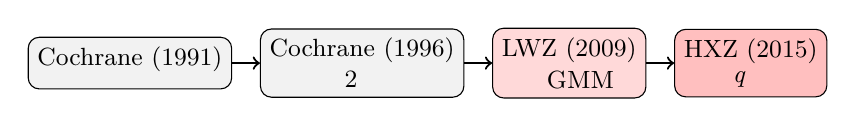
\begin{tikzpicture}[node distance=10pt, every node/.style={font=\small}]
            \node[draw,rounded corners,fill=gray!10] (a) {\shortstack{Cochrane (1991)\\时间序列}};
            \node[draw,rounded corners,fill=gray!10,right=of a] (b) {\shortstack{Cochrane (1996)\\2 因子}};
            \node[draw,rounded corners,fill=red!15,right=of b] (c) {\shortstack{LWZ (2009)\\结构 GMM}};
            \node[draw,rounded corners,fill=red!25,right=of c] (d) {\shortstack{HXZ (2015)\\\textit{q} 因子}};
            \draw[->,thick] (a) -- (b);
            \draw[->,thick] (b) -- (c);
            \draw[->,thick] (c) -- (d);
        \end{tikzpicture}
    \end{center}
\end{frame}

\section{Liu, Whited, and Zhang (2009)：使其经验化}

\begin{frame}{设定调整成本函数}
    \textbf{问题：}Q 理论给出一般关系，但经验研究需要具体形式

    \vspace{0.2cm}
    \textbf{\href{https://doi.org/10.1086/649760}{\textcolor{blue}{Liu, Whited, and Zhang (2009)}} 的设定：}
    \begin{equation}\label{equ:lwz cost}
        \phi\left(\frac{I_t}{K_t}\right) = \frac{I_t}{K_t} + \frac{a}{2}\left(\frac{I_t}{K_t}\right)^2
    \end{equation}

    其中 $a > 0$ 是调整成本参数


    \textbf{性质：}
    \begin{itemize}
        \item \textbf{购置成本：}$I_t/K_t$（仅购买资本）
        \item \textbf{二次调整成本：}$\frac{a}{2}(I_t/K_t)^2$（安装、扰动）
        \item \textbf{边际成本：}
        \begin{equation}\label{equ:marginal cost}
            \phi'\left(\frac{I_t}{K_t}\right) = 1 + a\left(\frac{I_t}{K_t}\right)
        \end{equation}
        \item 关于投资率线性：$\phi'$ 随 $I/K$ 线性增加
        \item \textbf{无调整成本时：}$a = 0 \Rightarrow \phi' = 1$（常数）
    \end{itemize}
\end{frame}

\begin{frame}{计算资本的边际价值}
    \textbf{由包络定理（\ref{equ:envelope theorem}）：}
    \begin{equation*}
        \frac{\partial V_{t+1}}{\partial K_{t+1}} = \alpha \frac{\partial Y_{t+1}}{\partial K_{t+1}} - \frac{\partial \Phi_{t+1}}{\partial K_{t+1}} + (1-\delta) \phi'\left(\frac{I_{t+1}}{K_{t+1}}\right)
    \end{equation*}

    \textbf{步骤 1：资本的边际产出}

    由于 $Y_t = Z_t^{1/\alpha} [(1-\alpha)/\omega_t]^{(1-\alpha)/\alpha} K_t$：
    \begin{equation*}
        \frac{\partial Y_{t+1}}{\partial K_{t+1}} = \frac{Y_{t+1}}{K_{t+1}}
    \end{equation*}

    \textbf{步骤 2：对调整成本的边际影响}

    由 $\Phi_t = \phi(I_t/K_t) K_t$：
    \begin{equation*}
        \begin{aligned}
            \frac{\partial \Phi_{t+1}}{\partial K_{t+1}} &= \phi\left(\frac{I_{t+1}}{K_{t+1}}\right) - \phi'\left(\frac{I_{t+1}}{K_{t+1}}\right) \frac{I_{t+1}}{K_{t+1}} \\
            &= \left[\frac{I_{t+1}}{K_{t+1}} + \frac{a}{2}\left(\frac{I_{t+1}}{K_{t+1}}\right)^2\right] - \left[1 + a\frac{I_{t+1}}{K_{t+1}}\right] \frac{I_{t+1}}{K_{t+1}} \\
            &= -\frac{a}{2}\left(\frac{I_{t+1}}{K_{t+1}}\right)^2
        \end{aligned}
    \end{equation*}
\end{frame}

\begin{frame}{完整的边际价值表达式}
    \textbf{综合所有项：}
    \begin{equation}\label{equ:marginal value}
        \boxed{
        \begin{aligned}
            \frac{\partial V_{t+1}}{\partial K_{t+1}} &= \alpha \frac{Y_{t+1}}{K_{t+1}} + \frac{a}{2}\left(\frac{I_{t+1}}{K_{t+1}}\right)^2 + (1-\delta)\left[1 + a\frac{I_{t+1}}{K_{t+1}}\right]
        \end{aligned}
        }
    \end{equation}


    \textbf{经济学解读——三个组成部分：}
    \begin{enumerate}
        \item $\alpha Y_{t+1}/K_{t+1}$：每单位资本的利润
        \begin{itemize}
            \item 更多资本的直接收益：更高产出 $\rightarrow$ 更高利润
        \end{itemize}

        \item $\frac{a}{2}(I_{t+1}/K_{t+1})^2$：调整成本节省
        \begin{itemize}
            \item 更大的资本基数 $\rightarrow$ 每单位调整成本更低
            \item 来自 $-\partial \Phi/\partial K < 0$（规模经济）
        \end{itemize}

        \item $(1-\delta)[1 + a(I_{t+1}/K_{t+1})]$：延续价值
        \begin{itemize}
            \item 未折旧资本存续至下期
            \item 价值为其边际安装成本
        \end{itemize}
    \end{enumerate}
\end{frame}

\begin{frame}{LWZ 收益率公式}
	由一阶条件，$1+R^I_{t+1}=(\partial V_{t+1}/\partial K_{t+1})/\phi'(I_t/K_t)$。代入边际价值（\ref{equ:marginal value}）与 $\phi'=1+a(I/K)$：
	\begin{equation}\label{equ:lwz return}
		\boxed{\,1+R^S_{t+1}=\frac{\overbrace{\alpha\,Y_{t+1}/K_{t+1}}^{\text{盈利能力}}+\overbrace{\tfrac a2(I_{t+1}/K_{t+1})^2+(1-\delta)\left[1+a\,I_{t+1}/K_{t+1}\right]}^{\text{资本演化}}}{\underbrace{1+a\,I_t/K_t}_{\text{今日投资成本}}}\,}
	\end{equation}
	\begin{itemize}
		\item 把\textbf{已实现收益率}与可观测会计数据 $Y/K,\ I/K$ 联系起来——无潜在 SDF。
		\item 只有\textbf{两个}结构参数：$\alpha$（资本份额）与 $a$（调整成本）。
		\item \textit{当盈利能力高且投资便宜（低 $I_t/K_t$）时收益率高}——这是两个预测的分子／分母重述。
	\end{itemize}
\end{frame}

\begin{frame}{LWZ 的经验策略：对矩做 GMM}
    \textbf{为何不逐状态检验强形式恒等式 $1+R^S_{t+1} = 1+R^I_{t+1}$？}
    \begin{itemize}
        \item 这样的精确约束被数据压倒性地拒绝。
        \item 由 $Y/K$、$I/K$ 的测量误差以及会计数据与市场数据之间的时点错配所致。
    \end{itemize}

    \vspace{0.2cm}
    \textbf{LWZ 的折中：匹配矩，而非路径。}
    \begin{itemize}
        \item 对每个检验组合 $i$，定义矩条件：
        \begin{equation*}
            g_i(\theta) = \begin{pmatrix} \mathrm{E}[R^S_{i,t+1}] - \mathrm{E}[R^I_{i,t+1}(\theta)] \\ \mathrm{Var}(R^S_{i,t+1}) - \mathrm{Var}(R^I_{i,t+1}(\theta)) \end{pmatrix}
        \end{equation*}
        其中 $\theta = (\alpha, a)$ 是仅有的结构参数。
        \item 用 \textbf{GMM} 跨组合最小化 $\{g_i(\theta)\}$ 的加权范数。
    \end{itemize}

    \vspace{0.1cm}
    \textbf{为何这是简约的：}两个参数同时约束收益率\textit{均值与波动率}的横截面。无潜在因子，无偏好参数。
\end{frame}

\begin{frame}{LWZ 的检验资产与主要发现}
    \textbf{三组检验组合（各捕捉一个异象）：}
    \begin{enumerate}
        \item \textbf{按资本投资排序：}高 $I/A$ 企业平均收益率低（\href{https://doi.org/10.1111/j.1540-6261.2004.00709.x}{\textcolor{blue}{Titman, Wei, Xie 2004}}）。
        \item \textbf{按盈余惊喜排序（SUE）：}盈余公告后漂移——高 SUE 企业持续跑赢。
        \item \textbf{按账面市值比排序：}经典的价值溢价。
    \end{enumerate}

    \vspace{0.2cm}
    \textbf{不同组合类型下估计的参数 $(\alpha, a)$：}
    \small
    \begin{center}
        \begin{tabular}{@{}lcc@{}}
            \toprule
            \textbf{组合排序} & $\alpha$（资本份额） & $a$（调整成本） \\
            \midrule
            投资 $I/A$ & $0.2$--$0.5$ & \textbf{低} \\
            盈余惊喜（SUE） & $0.2$--$0.5$ & 中等 \\
            账面市值比 & $0.2$--$0.5$ & \textbf{非常高} \\
            \bottomrule
        \end{tabular}
    \end{center}

    \vspace{0.1cm}
    \textbf{解读。}
    \begin{itemize}
        \item 资本份额合理且在各异象间稳定。
        \item 但调整成本参数\textit{并非如此}：对价值型企业，它必须远高于按投资排序的企业。
    \end{itemize}
\end{frame}

\begin{frame}{为何不同异象需要不同的 $a$}
    \textbf{LWZ 公式（\ref{equ:lwz return}）的机理：}
    \begin{equation*}
        1 + R^S_{t+1} = \frac{\alpha\, Y_{t+1}/K_{t+1} + \frac{a}{2}(I_{t+1}/K_{t+1})^2 + (1-\delta)[1+a(I_{t+1}/K_{t+1})]}{1 + a(I_t/K_t)}
    \end{equation*}

    \vspace{0.1cm}
    \textbf{按投资排序（低 $a$ 即可）：}
    \begin{itemize}
        \item 高投资企业\textit{今日}的 $I_t/K_t$ 非常高，但明日的 $I_{t+1}/K_{t+1}$ 低得多。
        \item 一个适度为正的 $a$ 已通过分母拉低其收益率。过大的 $a$ 会矫枉过正。
    \end{itemize}

    \vspace{0.15cm}
    \textbf{按价值排序（需要非常高的 $a$）：}
    \begin{itemize}
        \item 成长型企业在\textit{两期}都有高投资，且 $Y/K$ 高。
        \item 若没有大的 $a$，公式会预测成长型企业有\textit{高}收益率——与数据相反。
        \item 迫使 $a$ 大到使凸成本主导盈利项。
    \end{itemize}

    \vspace{0.15cm}
    \begin{block}{普遍存在的异质性问题}
        “不同异象用不同参数”是 $q$ 理论资产定价的一种慢性病。更干净的经验应对是 HXZ 的 \textit{q} 因子模型，它用模拟组合的载荷取代结构估计。
    \end{block}
\end{frame}

\section{经验含义与预测}

\begin{frame}{为何投资能预测收益率：三种渠道}
    \textbf{渠道 1：资本的边际报酬递减}
    \begin{itemize}
        \item 今日大量投资 $\rightarrow$ 明日更多资本
        \item 更多资本 $\rightarrow$ 更低的边际生产率（报酬递减）
        \item 更低的生产率 $\rightarrow$ 更低的未来利润
        \item 更低的利润 $\rightarrow$ 更低的收益率
    \end{itemize}

    \vspace{0.2cm}
    \textbf{渠道 2：时变折现率}
    \begin{itemize}
        \item 当折现率（要求收益率）低时企业投资更多
        \item 当前折现率低 $\rightarrow$ 未来已实现收益率低
        \item 理性：在资本“便宜”（低 $r$）时投资是最优的
    \end{itemize}

    \vspace{0.2cm}
    \textbf{渠道 3：投资成本}
    \begin{itemize}
        \item 高 $I/K$ 意味着高边际成本 $\phi'$
        \item 收益率 = 收益 / 成本
        \item 高成本 $\rightarrow$ 每投资一美元的收益率更低
        \item 来自凸调整成本的纯机械效应
    \end{itemize}

    \vspace{0.2cm}
    \textit{三种渠道方向一致：高投资 $\rightarrow$ 低收益率}
\end{frame}

\begin{frame}{与 Fama-French 因子的关系}
    \textbf{\href{https://doi.org/10.1016/j.jfineco.2014.10.010}{\textcolor{blue}{Fama-French 五因子模型（2015）}}：} 2014.10
    \begin{equation*}
    \begin{aligned}
        R_i - R_f &= \alpha + \beta_{MKT}(R_M - R_f) + \beta_{SMB}SMB + \beta_{HML}HML \\
        &+ \beta_{RMW}RMW + \beta_{CMA}CMA
    \end{aligned}
    \end{equation*}

    \textbf{基于生产的解读：}
    \begin{itemize}
        \item \textbf{RMW（稳健减疲弱）：}盈利因子
        \begin{itemize}
            \item 做多高营业盈利、做空低盈利
            \item 与生产模型中的 $Y/K$ 直接相关
        \end{itemize}

        \item \textbf{CMA（保守减激进）：}投资因子
        \begin{itemize}
            \item 做多低投资企业、做空高投资企业
            \item 与生产模型中的 $I/K$ 直接相关
        \end{itemize}
    \end{itemize}
\end{frame}

\section{解释企业的 Beta：Zhang (2005)}

\begin{frame}{从定价到 Beta：一个不同的问题}
    \textbf{至此：}我们用投资 + 盈利\textit{特征}为横截面定价。

    \vspace{0.2cm}
    \textbf{现在问：}为何\textit{价值型}企业比\textit{成长型}企业\textbf{与 SDF 的协动更强}？
    \begin{itemize}
        \item 这就是最初的 Fama-French (1992) 价值溢价之谜。
        \item 经验上：高 B/M（价值）企业平均收益率更高，在某些时期 beta 也更高。
        \item 挑战：用带有外生 SDF 的生产模型\textbf{内生地产生}价值溢价。
    \end{itemize}

    \vspace{0.2cm}
    \textbf{\href{https://doi.org/10.1111/j.1540-6261.2004.00709.x}{\textcolor{blue}{Zhang (2005, JF)}}：“价值溢价”}
    \begin{itemize}
        \item 取一个异方差的单因子 SDF 为给定（排除行为渠道）。
        \item 加入\textbf{非对称}调整成本：撤资比投资代价更高。
        \item 证明这种非对称性内生地产生可观的价值溢价。
    \end{itemize}
\end{frame}

\begin{frame}{Zhang (2005)：SDF 与生产率}
    \textbf{异方差单因子 SDF（对数形式）：}
    \begin{equation}\label{equ:zhang sdf}
        m_{t+1} = \log\beta - \gamma_t (x_{t+1} - x_t)
    \end{equation}
    \begin{equation}\label{equ:zhang gamma}
        \gamma_t = \gamma_0 + \gamma_1 (x_t - \bar{x}), \qquad \gamma_1 < 0
    \end{equation}
    其中 $x_t$ 是服从 AR(1) 的总量（对数）生产率。

    \textbf{解读。}风险价格 $\gamma_t$ 在坏时期（$x_t$ 低）上升——内嵌了逆周期的风险厌恶。

    \vspace{0.2cm}
    \textbf{企业 $j$ 的特质生产率：}
    \begin{itemize}
        \item $z_{jt}$ 服从具有共同持续性的 AR(1)。
        \item \textbf{价值型}企业：当前 $z_{jt}$ 低 $\rightarrow$ 低生产率、低投资、低利润。
        \item \textbf{成长型}企业：当前 $z_{jt}$ 高 $\rightarrow$ 高生产率、高投资。
    \end{itemize}

    \vspace{0.2cm}
    \textbf{条件 CAPM 按构造成立}，但模型仍产生可观的\textit{无条件}价值溢价。
\end{frame}

\begin{frame}{非对称调整成本}
    \textbf{二次但在 $I=0$ 处有拐折：}
    \begin{equation}\label{equ:zhang cost}
        \phi_{jt} = \frac{I_{jt}}{K_{jt}} + \frac{a_{jt}}{2}\left(\frac{I_{jt}}{K_{jt}}\right)^2,
        \qquad a_{jt} = \begin{cases} a^+ & \text{若 } I_{jt} > 0 \\ a^- & \text{若 } I_{jt} < 0 \end{cases}
    \end{equation}
    以及核心约束
    \begin{equation*}
        \boxed{a^- > a^+}
    \end{equation*}

    \vspace{0.1cm}
    \textbf{为何这种非对称是现实的。}
    \begin{itemize}
        \item 二手资本市场缺乏流动性；转售已安装资本会有很大折价。
        \item 裁员与重组成本集中在撤资一侧。
        \item 专用人力资本、干中学以及合约刚性都造成向下的不灵活性。
    \end{itemize}

    \vspace{0.1cm}
    \textbf{微观经验证据：}\href{https://doi.org/10.1086/250002}{\textcolor{blue}{Caballero, Engel, Haltiwanger (1995)}}；\href{https://www.jstor.org/stable/2233834}{\textcolor{blue}{Cooper-Haltiwanger (2006)}}。
\end{frame}

\begin{frame}{机制：谁承担坏时期的风险？}
    \textbf{校准结果。}
    \begin{itemize}
        \item 在好时期：价值型与成长型企业都投资，但\textbf{成长型投资更多} $\rightarrow$ 在边际上支付较高的 $a^+$。
        \item 在坏时期：成长型仍适度投资，但\textbf{价值型撤资} $\rightarrow$ 在边际上支付高得多的 $a^-$。
    \end{itemize}

    \vspace{0.2cm}
    \begin{center}
        \small
        \begin{tabular}{@{}lcc@{}}
            \toprule
            & \textbf{好时期} & \textbf{坏时期} \\
            \midrule
            \textbf{成长型}（高 $z_j$） & 高 $I/K$、高 $a^+$ 成本 & 中等 $I/K$、$a^+$ 成本 \\
            \textbf{价值型}（低 $z_j$） & 中等 $I/K$、$a^+$ 成本 & 撤资、\textbf{高 $a^-$ 成本} \\
            \bottomrule
        \end{tabular}
    \end{center}

    \vspace{0.2cm}
    \textbf{对风险的含义：}
    \begin{itemize}
        \item 在边际上调整成本\textbf{低}的企业能平滑股利 $\rightarrow$ 风险更低。
        \item 调整成本\textbf{高}的企业无法平滑 $\rightarrow$ 风险更高。
        \item \textbf{成长型}企业在\textit{好}时期更具风险；\textbf{价值型}企业在\textit{坏}时期更具风险。
    \end{itemize}
\end{frame}

\begin{frame}{为何会出现无条件价值溢价}
    \textbf{把非对称暴露与异方差 SDF 结合：}
    \begin{itemize}
        \item 价值型企业恰好在风险价格 $\gamma_t$ \textit{高}（坏时期）时具有风险。
        \item 成长型企业在风险价格\textit{低}（好时期）时具有风险。
        \item 无条件预期收益率：$\mathrm{E}[R_j] - R_f \approx -\mathrm{Cov}(M_{t+1}, R_{j,t+1})$。
        \item 若协方差落在高 $\gamma_t$ 状态，同样的 $\beta$ 会获得更高回报。
    \end{itemize}

    \vspace{0.2cm}
    \begin{equation*}
        \underbrace{\mathrm{E}[R^V] - \mathrm{E}[R^G]}_{\text{价值溢价}} > 0
        \;\;\Leftarrow\;\;
        \underbrace{\text{价值型在坏时期的风险}}_{\text{高风险价格}}
        \;>\;
        \underbrace{\text{成长型在好时期的风险}}_{\text{低风险价格}}
    \end{equation*}

    \vspace{0.1cm}
    \begin{block}{要点}
        生产技术 + 非对称调整成本，足以从外生 SDF 中\textbf{内生化}出价值溢价，而无需诉诸行为性错误定价。
    \end{block}
\end{frame}

\begin{frame}{局限与现代扩展}
    \textbf{Zhang (2005) 无法给出的：}
    \begin{itemize}
        \item 按构造强加\textbf{条件 CAPM} $\rightarrow$ 只能产生\textit{很小}的无条件 CAPM-alpha。
        \item 无法匹配 1990 年代后的证据：价值型企业的 CAPM beta \textbf{低于}成长型企业。
        \item 对动量及其他非价值异象保持沉默。
    \end{itemize}

    \vspace{0.2cm}
    \textbf{推广（更偏离 CAPM 的替代 SDF）：}
    \begin{itemize}
        \item \href{https://doi.org/10.1093/rfs/hht067}{\textcolor{blue}{Bazdresch, Belo, Lin (2014)}}：调整成本的冲击。
        \item \href{https://doi.org/10.1111/jofi.12080}{\textcolor{blue}{Kogan and Papanikolaou (2014)}}：投资专用技术冲击降低投资品价格；成长期权提供保险。
        \item \href{https://doi.org/10.1093/rfs/hhx135}{\textcolor{blue}{McQuade (2018)}}：正向波动率冲击提高边际效用；成长型企业对其进行对冲。
    \end{itemize}

    \vspace{0.1cm}
    \textbf{共同线索。}超越 CAPM 式的 SDF，以捕捉成长期权的保险价值或对特定冲击类型的厌恶。
\end{frame}

\section{$q$ 因子模型：Hou--Xue--Zhang (2015) 与 $q^5$}

\begin{frame}{张橹的研究纲领：从 Cochrane (1991) 到 $q^5$}
	\small
	一个研究纲领，三十年，一个理念——\textit{金融收益率等于投资收益率}：
	\begin{enumerate}
		\item \textbf{1991} \quad \href{https://doi.org/10.1111/j.1540-6261.1991.tb03750.x}{\textcolor{blue}{Cochrane (JF)}}：基于生产的资产定价；总量层面的恒等式 $R^S=R^I$。
		\item \textbf{2009} \quad \href{https://doi.org/10.1086/649760}{\textcolor{blue}{Liu--Whited--Zhang (JPE)}}：结构 GMM 从投资一阶条件出发，为投资、价值与盈余惊喜组合定价。
		\item \textbf{2015} \quad \href{https://doi.org/10.1093/rfs/hhu068}{\textcolor{blue}{Hou--Xue--Zhang (RFS)}}：可交易的 \textbf{$q$ 因子模型}——MKT、ME、I/A、ROE。
		\item \textbf{2021} \quad \href{https://doi.org/10.1093/rof/rfaa004}{\textcolor{blue}{HMXZ (RoF)}}：$q^5$ 加入动态一阶条件所预测的\textbf{预期增长}因子。
	\end{enumerate}
	\vspace{2pt}
	{\footnotesize\textit{旁注。}这篇 2015 RFS 论文最初是 2009 年一篇被 JF 接收的“更好的三因子模型”，后因一个时点错误被撤回，修订后又遭拒；团队重建模型，并在 FF5 问世的同一年发表于 RFS。\textbf{完整的因子战争故事属于第 07 讲。}}
\end{frame}

\begin{frame}{HXZ (2015)：投资一阶条件的运用}
	\textbf{两期经济，二次成本}（用账面资产 $A$ 代理资本存量 $K$，故 $I/K\to I/A$）。企业 $i$ 的一阶条件令边际成本等于预期边际收益，$1+a\,I_{i0}/A_{i0}=\mathrm{E}_0[M_1\,(\Pi_{i1}/A_{i1}+(1-\delta))]$，在规模报酬不变下，股票毛收益率坍缩为
	\[
		1+R^S_{i,1}=\frac{\Pi_{i,1}/A_{i,1}+(1-\delta)}{1+a\,I_{i,0}/A_{i,0}}\ \Longrightarrow\ \mathrm{E}_0[1+R^S_{i,1}]=\frac{\mathrm{E}_0[\Pi_{i,1}/A_{i,1}]+(1-\delta)}{1+a\,I_{i,0}/A_{i,0}},
	\]
	这是核心方程（\ref{equ:investment capm}）的经验对应物。两个预测成为两个非市场因子：
	\begin{itemize}
		\item 高 $I/A \Rightarrow$ 低预期收益率 $\Rightarrow$ \textbf{I/A} 因子（低投资减高投资）。
		\item 高预期盈利 $\Rightarrow$ 高预期收益率 $\Rightarrow$ \textbf{ROE} 因子。
	\end{itemize}
	\begin{block}{为何这优于会计恒等式}
		HXZ 的因子是把最优投资法则投影到可观测特征上的产物——\textit{事前}从企业最优化推导出来，而非\textit{事后}打补丁拼到 FF3 上。
	\end{block}
\end{frame}

\begin{frame}{构造四个 \textit{q} 因子}
	\small
	\textbf{变量。}
	\begin{itemize}
		\item \textbf{ME} $=$ 价格 $\times$ 股数（CRSP，6 月末）。
		\item \textbf{I/A} $=\Delta\text{AT}/\text{AT}_{-1}$（Compustat 年度）。
		\item \textbf{ROE} $=\text{IBQ}_q/\text{账面权益}_{q-1}$（Compustat 季度，\textit{按月}更新）。
	\end{itemize}
	\textbf{三重 $2\times3\times3$ 排序}（纽交所断点），1972 至今，剔除金融业：
	\begin{itemize}
		\item 规模：纽交所中位数 $\to$ 2 组（6 月末）。
		\item I/A：30/40/30 $\to$ 3 组（6 月末，财年 $t-1$）。
		\item ROE：30/40/30 $\to$ 3 组，\textit{每月}用最新盈余重新计算。
	\end{itemize}
	$\Rightarrow$ 18 个组合；因子为角组合均值：$r_{\text{ME}}$（小$-$大）、$r_{\text{I/A}}$（低$-$高）、$r_{\text{ROE}}$（高$-$低）。
	\begin{block}{时点修正（2010 年时点错误的教训）}
		ROE \textbf{仅在}公开公告日（Compustat \texttt{RDQ}）\textbf{之后}才使用盈余，而非一刀切地滞后 4 个月。基于实时盈余的\textit{按月}ROE 再平衡，正是 $q$ 因子能吸收\textbf{动量}、而按年更新的 FF5 不能的原因。
	\end{block}
\end{frame}

\begin{frame}{HXZ 经验要点：异象受审}
	\small
	\textbf{样本}（1972--2012）：在约 80 个候选异象中，采用纽交所断点与市值加权后约\textbf{一半不显著}。在存活的约 35 个中：
	\begin{center}
		\footnotesize
		\begin{tabular}{lccc}
			\toprule
			模型 & $\overline{|\alpha_{H{-}L}|}$ & \#\{$|t|>1.96$\} & GRS 拒绝 \\
			\midrule
			FF3 & 0.55\% & 27 & 28 \\
			Carhart 4 & 0.33\% & 19 & 24 \\
			\textbf{Q4 (HXZ)} & \textbf{0.20\%} & \textbf{5} & \textbf{20} \\
			\bottomrule
		\end{tabular}
	\end{center}
	\textbf{Q4 大胜}于动量（经由 ROE）、盈利（ROE），以及净发行／应计／综合发行（经由 I/A）。\quad \textbf{Q4 吃力}于营业应计与 R\&D 市值比——R\&D 的 GAAP 费用化压低了创新者的 ROE。
	\begin{block}{结构化的回报}
		一个从投资一阶条件\textit{推导}出的四因子模型，匹配甚至击败经验挖掘的 Carhart 模型——这是“驱动横截面的是生产纪律而非数据挖掘”的最干净证据。
	\end{block}
\end{frame}

\begin{frame}{为何需要第五个因子？从静态坍缩到动态收益率}
	\textbf{Q4 遗漏了什么。}HXZ 的\textbf{静态}坍缩只用两个特征——投资与预期盈利。但在约 150 个显著异象中，仍有 \textbf{52 个无法被 $q$ 因子模型定价}：R\&D 市值比、营业与可操控应计、盈余公告漂移……
	\vspace{2pt}
	\textbf{修复：不要坍缩延续项。}两期模型在 $t+1$ 清算（$I_{t+1}=0$），杀死了延续项。恢复折旧 $\delta<1$ 与无限期：把完整的包络结论（\ref{equ:envelope theorem}，二次成本下 $\phi'=1+a\,I/A$）代回中心恒等式（\ref{equ:central identity}），\textit{保留} $I_{t+1}\neq0$：
	\begin{equation}\label{equ:q5 dynamic ir}
		\resizebox{\linewidth}{!}{$\displaystyle
		\boxed{\,1+R^S_{i,t+1}=\frac{\Pi_{i,t+1}/A_{i,t+1}+\tfrac a2(I_{i,t+1}/A_{i,t+1})^2+(1-\delta)\big[1+a\,(I_{i,t+1}/A_{i,t+1})\big]}{1+a\,(I_{i,t}/A_{i,t})}\,}
		$}
	\end{equation}
	{\footnotesize 令\textbf{下期}投资 $I_{i,t+1}=0$，分子坍缩回 $\Pi/A+1-\delta$，即静态投资 CAPM（\ref{equ:investment capm}）——所有新内容都在残留的 $I_{i,t+1}/A_{i,t+1}$ 项里。} \href{https://doi.org/10.1093/rof/rfaa004}{\textcolor{blue}{HMXZ (2021, RoF)}} 的 $q^5$ 即源于此。
\end{frame}

\begin{frame}{三个决定因素：解读横截面}
	\textbf{把（\ref{equ:q5 dynamic ir}）拆成“股利收益率”与“资本利得”：}
	\[
		1+R^S_{i,t+1}=\underbrace{\frac{\Pi_{i,t+1}/A_{i,t+1}+\tfrac a2(I_{i,t+1}/A_{i,t+1})^2}{1+a\,(I_{i,t}/A_{i,t})}}_{\text{股利收益率}\,\approx\,\text{静态模型}}+\underbrace{\frac{(1-\delta)\big(1+a\,I_{i,t+1}/A_{i,t+1}\big)}{1+a\,(I_{i,t}/A_{i,t})}}_{\text{资本利得}\,=\,\text{边际 }q\text{ 的增长}}.
	\]
	\begin{itemize}
		\item \textbf{股利收益率}——平方项在经济上极小，故这一块复刻了静态的\textbf{投资}与\textbf{盈利}两渠道。
		\item \textbf{资本利得}——边际 $q$ 的增长，近似正比于\textbf{投资率增长} $\dfrac{I_{i,t+1}/A_{i,t+1}}{I_{i,t}/A_{i,t}}$（Cochrane 1991）。
	\end{itemize}
	\begin{block}{预期收益率现在有\emph{三个}决定因素}
		它随（i）\textbf{低}投资 $I_{it}/A_{it}$、（ii）\textbf{高}预期盈利 $\mathrm{E}_t[\Pi_{i,t+1}/A_{i,t+1}]$、以及如今的（iii）\textbf{高}预期投资增长而上升。
	\end{block}
\end{frame}

\begin{frame}{预期增长渠道——经济学}
	\textbf{命题。}固定投资 $I_{it}/A_{it}$ 与预期盈利，\textbf{预期收益率随预期投资增长上升}。
	\vspace{3pt}
	\textbf{为什么。}项 $1+a\,I_{i,t+1}/A_{i,t+1}$ 是\textbf{下期}投资的边际成本，按投资第一性原理，它等于\textbf{下期的边际 $q$}——即下期新增一单位资产所带来的全部未来现金流的现值。而它本身又是\textit{今日}投资边际收益的一部分。
	\begin{block}{折现率逻辑（与盈利渠道完全平行）}
		若下期预期投资相对当期\textbf{高}，则今日投资的边际收益高。要使我们固定的\textbf{低当期投资}合理化，\textbf{折现率必须高}以抵消之。
	\end{block}
	{\footnotesize \textbf{盈利渠道：}高 $\mathrm{E}[\Pi/A]$ 配低 $I/A$ $\Rightarrow$ 高折现率。\quad \textbf{增长渠道：}高预期投资增长配低 $I/A$ $\Rightarrow$ 高折现率。同样的净现值逻辑，只是向后多推一期。}
\end{frame}

\begin{frame}[allowframebreaks]{从理论到因子：估计预期增长}
	投资 $I/A$ 与盈利 ROE 是\textbf{可观测}的；预期投资增长\textbf{不可观测}，必须\textbf{预测}。
	\begin{itemize}
		\item \textbf{预测变化而非增长率。}企业层面 $I/A$（净资产增长）常为负，增长\textit{率}无定义。改为预测未来\textbf{投资率变化} $\Delta^\tau I/A$（第 $t{+}\tau$ 财年的 $I/A$ 减当期 $I/A$），$\tau=1,2,3$。
		\item \textbf{方法。}按月 \textbf{Fama--MacBeth} 横截面回归；预期变化 $\mathrm{E}_t[\Delta^\tau I/A]$ 用最新预测变量乘以\textbf{120 个月滚动窗口}的平均斜率。
	\end{itemize}
	\textbf{三个预测变量，各有概念依据：}
	\begin{itemize}
		\item \textbf{托宾 $q$（$\log q$）：}Hayashi——边际 $q$ 驱动投资。但单独使用\textbf{很弱}（$R^2\approx1\%$）。
		\item \textbf{营业现金流 $C^{op}$}（\href{https://doi.org/10.1016/j.jfineco.2016.03.002}{\textcolor{blue}{Ball 等 2016}}）：内部资金越多投资越多；并捕捉\textbf{无形资产}（R\&D 等被费用化，使盈利低估增长）。\textbf{关键预测变量。}
		\item \textbf{ROE 变化（$\Delta$ROE）：}近期盈利改善的企业会提高近期投资（短期动态）。
	\end{itemize}
	\break
	\textbf{$\Delta^1 I/A$ 的基准预测回归}（WLS，按月，1963--2018）：
	\begin{center}
		\small
		\begin{tabular}{@{}lcccc@{}}
			\toprule
			& $\log q$ & $C^{op}$ & $\Delta$ROE & $R^2$ \\
			\midrule
			斜率 & $-0.03$ & $0.52$ & $0.77$ & $6.4\%$ \\
			$t$  & $(-5.6)$ & $(12.8)$ & $(7.6)$ & \\
			\bottomrule
		\end{tabular}
	\end{center}
	拟合的 $\mathrm{E}_t[\Delta^1 I/A]$ 与随后\textbf{实现}的变化高度吻合：组合层面预期与实现的变化都从约 $-16\%$（第 1 组）到约 $+7\%$（第 10 组），横截面相关系数 $0.64$。
\end{frame}

\begin{frame}{预期增长因子 $R_{\text{Eg}}$}
	\textbf{构造}（Fama--French 流程）：按\textbf{规模}与\textbf{预期 1 年期增长} $\mathrm{E}_t[\Delta^1 I/A]$ 做独立 $2\times3$ 排序（纽交所 30/40/30 断点，市值加权）；$R_{\text{Eg}}=$ 高 $-$ 低。
	\begin{center}
		\small
		\begin{tabular}{@{}lcc@{}}
			\toprule
			$R_{\text{Eg}}$，按月 1967--2018 & 估计值 & $t$ \\
			\midrule
			平均溢价                       & $0.84\%$ & $(10.27)$ \\
			$q$ 因子 alpha                 & $0.67\%$ & $(9.75)$ \\
			\quad 对 $R_{I/A}$ 的载荷       & $0.21$   & $(4.86)$ \\
			\quad 对 $R_{\text{ROE}}$ 的载荷 & $0.30$   & $(9.13)$ \\
			\bottomrule
		\end{tabular}
	\end{center}
	\begin{itemize}
		\item 溢价 $t=10.27$ 远超 Harvey--Liu--Zhu（$t>3$）的多重检验门槛。
		\item $q$ 因子模型\textbf{无法}张成它（$\alpha=0.67\%$）：一个全新的收益率维度。
		\item \textbf{$C^{op}$ 是引擎：}向 $q$ 加入现金流因子后，$R_{\text{Eg}}$ 的 alpha 降到 $0.37\%$；$\log q$ 与 $\Delta$ROE 单独贡献甚微。
	\end{itemize}
\end{frame}

\begin{frame}{$q^5$ 模型}
	\textbf{在四个 $q$ 因子上加入预期增长因子：}
	\begin{equation}\label{equ:q5model}
		\resizebox{\linewidth}{!}{$\displaystyle
		\mathrm{E}[R_i]-R_f=\beta^i_{\text{Mkt}}\mathrm{E}[R_{\text{Mkt}}]+\beta^i_{\text{Me}}\mathrm{E}[R_{\text{Me}}]+\beta^i_{I/A}\mathrm{E}[R_{I/A}]+\beta^i_{\text{ROE}}\mathrm{E}[R_{\text{ROE}}]+\beta^i_{\text{Eg}}\mathrm{E}[R_{\text{Eg}}]
		$}
	\end{equation}
	前四个因子与 $q$ 因子模型\textbf{完全相同}；只有 $R_{\text{Eg}}$ 是新的。
	\begin{block}{张成判决——最大月度夏普比率（原文表 V）}
		\begin{center}
			\small
			\begin{tabular}{@{}cccccc@{}}
				\toprule
				$q^5$ & BS6 & FF6c & $q$ & FF6 & FF5 \\
				\midrule
				\textbf{0.63} & 0.48 & 0.43 & 0.42 & 0.37 & 0.32 \\
				\bottomrule
			\end{tabular}
		\end{center}
		$R_{\text{Eg}}$ 单独就拥有全研究中\textbf{最高}的个体夏普比率 $0.44$。
	\end{block}
\end{frame}

\begin{frame}{横向比较：150 个异象}
	\textbf{检验资产：}采用纽交所断点与市值加权后显著的 150 个异象（HXZ 2019，《复制异象》）。$q^5$ 是\textbf{总体最佳}。
	\begin{center}
		\small
		\begin{tabular}{@{}lccccc@{}}
			\toprule
			150 个高$-$低组合 & $q^5$ & $q$ & FF6 & FF6c & SY4 \\
			\midrule
			$\overline{|\alpha_{H-L}|}$（\%/月） & \textbf{0.19} & 0.28 & 0.30 & 0.27 & 0.29 \\
			\#\{$|t|\ge1.96$\}                  & \textbf{23}   & 52   & 74   & 59   & 64 \\
			\#\{$|t|\ge3$\}                     & \textbf{6}    & 25   & 37   & 25   & 25 \\
			GRS 拒绝数（共 150）                 & \textbf{57}   & 101  & 91   & 71   & 87 \\
			\bottomrule
		\end{tabular}
	\end{center}
	\begin{itemize}
		\item 仅加\textbf{一个}因子，就把 $q$ 模型无法解释的异象减半（$52\to23$）。
		\item 在\textbf{投资}与\textbf{盈利}两类收益最大；动量被进一步消化（ROE $+$ EG）。
		\item $q^5$ 在\textit{每一项}指标上都胜过 Fama--French 六因子模型（即便换成 $RMW_c$）。
	\end{itemize}
\end{frame}

\begin{frame}{预期增长修复了什么}
	\textbf{击垮 $q$ 模型的异象，恰恰是由增长驱动的那些}（高$-$低 $\alpha$ 单位 \%/月，括号内为 $t$）：
	\begin{center}
		\small
		\begin{tabular}{@{}lccc@{}}
			\toprule
			高$-$低组合 & $\alpha_q$ & $\alpha_{q^5}$ & $\beta_{\text{Eg}}$ \\
			\midrule
			R\&D 市值比（Rdm）       & $0.81\ (3.6)$   & $0.27\ (1.2)$   & $+0.84$ \\
			营业应计（Oa）           & $-0.57\ (-4.3)$ & $-0.20\ (-1.3)$ & $-0.56$ \\
			可操控应计（Dac）        & $-0.74\ (-5.3)$ & $-0.31\ (-2.2)$ & $-0.64$ \\
			净金融资产变化（dFin）   & $0.41\ (3.0)$   & $0.14\ (1.0)$   & $+0.40$ \\
			\bottomrule
		\end{tabular}
	\end{center}
	\begin{itemize}
		\item \textbf{R\&D：}当期费用化 $\Rightarrow$ 压低当期盈利，但积累无形资本 $\Rightarrow$ \textbf{高}未来增长 $\Rightarrow$ $\beta_{\text{Eg}}>0$。
		\item \textbf{应计：}给定盈利，高应计意味着\textbf{低现金流} $\Rightarrow$ 内部资金少 $\Rightarrow$ \textbf{低}预期增长 $\Rightarrow$ $\beta_{\text{Eg}}<0$。
	\end{itemize}
	{\footnotesize 有一个异象\textit{所有}模型都无法解释——盈余公告前后的收益（Abr）：$\alpha_{q^5}=0.52\%$（$t=3.8$）。}
\end{frame}

\begin{frame}{解读与一个警示}
	\begin{block}{维度缩减，而非（必然的）风险故事}
		HMXZ 把 $q^5$ 解读为对（\ref{equ:q5 dynamic ir}）这一非线性企业层面资本成本的\textbf{线性近似}——一个\textbf{降维}工具（Cochrane 2011），而非已定价风险的主张。该证据\textbf{与错误定价并不矛盾}（例如市场低估无形资产，Edmans 2011）。
	\end{block}
	\textbf{诚实的警示。}与 $I/A$ 和 ROE 不同，预期增长是\textbf{构造}出来的：它依赖于预测变量清单，\textbf{尤其依赖营业现金流 $C^{op}$}。去掉 $C^{op}$，因子就会减弱。作者也呼应了 Fama--French 对“经验上稳健却缺乏理论动机”的因子的担忧。
	\vspace{2pt}
	\textit{尽管如此：}$t=10.27$ 的溢价跨过了一切多重检验门槛，而“现金流 $\to$ 增长”的联系扎根于深厚的会计文献（Ball 等 2016；Lev \& Gu 2016）。
\end{frame}

\begin{frame}{收尾：第 06 讲交付了什么，以及向第 07 讲的交接}
	\textbf{主线，三行概括。}
	\begin{enumerate}
		\item 企业最优化 $\Rightarrow$ 投资收益率 $\Rightarrow$ $R^S=R^I$（Cochrane 恒等式）。
		\item 坍缩 $\Rightarrow$ $\mathrm{E}_t[1+R^S]=\dfrac{\text{预期盈利能力}}{1+a\,(I/K)}$（投资 CAPM）。
		\item 解读横截面 $\Rightarrow$ I/A、ROE 与预期增长 $\Rightarrow$ $q$ 因子模型及其增广版本 $q^5$。
	\end{enumerate}
	\vspace{4pt}
	\begin{block}{向第 07 讲的交接}
		\textit{哪个}模型胜出——FF5 与 Q4 的张成检验、夏普比率平方、HML 的冗余、正式的横向比较（\href{https://doi.org/10.1093/rof/rfy032}{\textcolor{blue}{HMXZ 2019}}），以及更广义的因子动物园／因子战争——是第 07 讲的主题。这里我们只搭建了那个结构化的挑战者。
	\end{block}
\end{frame}

\begin{frame}{$q$ 阵营的宣言}
	\begin{figure}
		\centering
		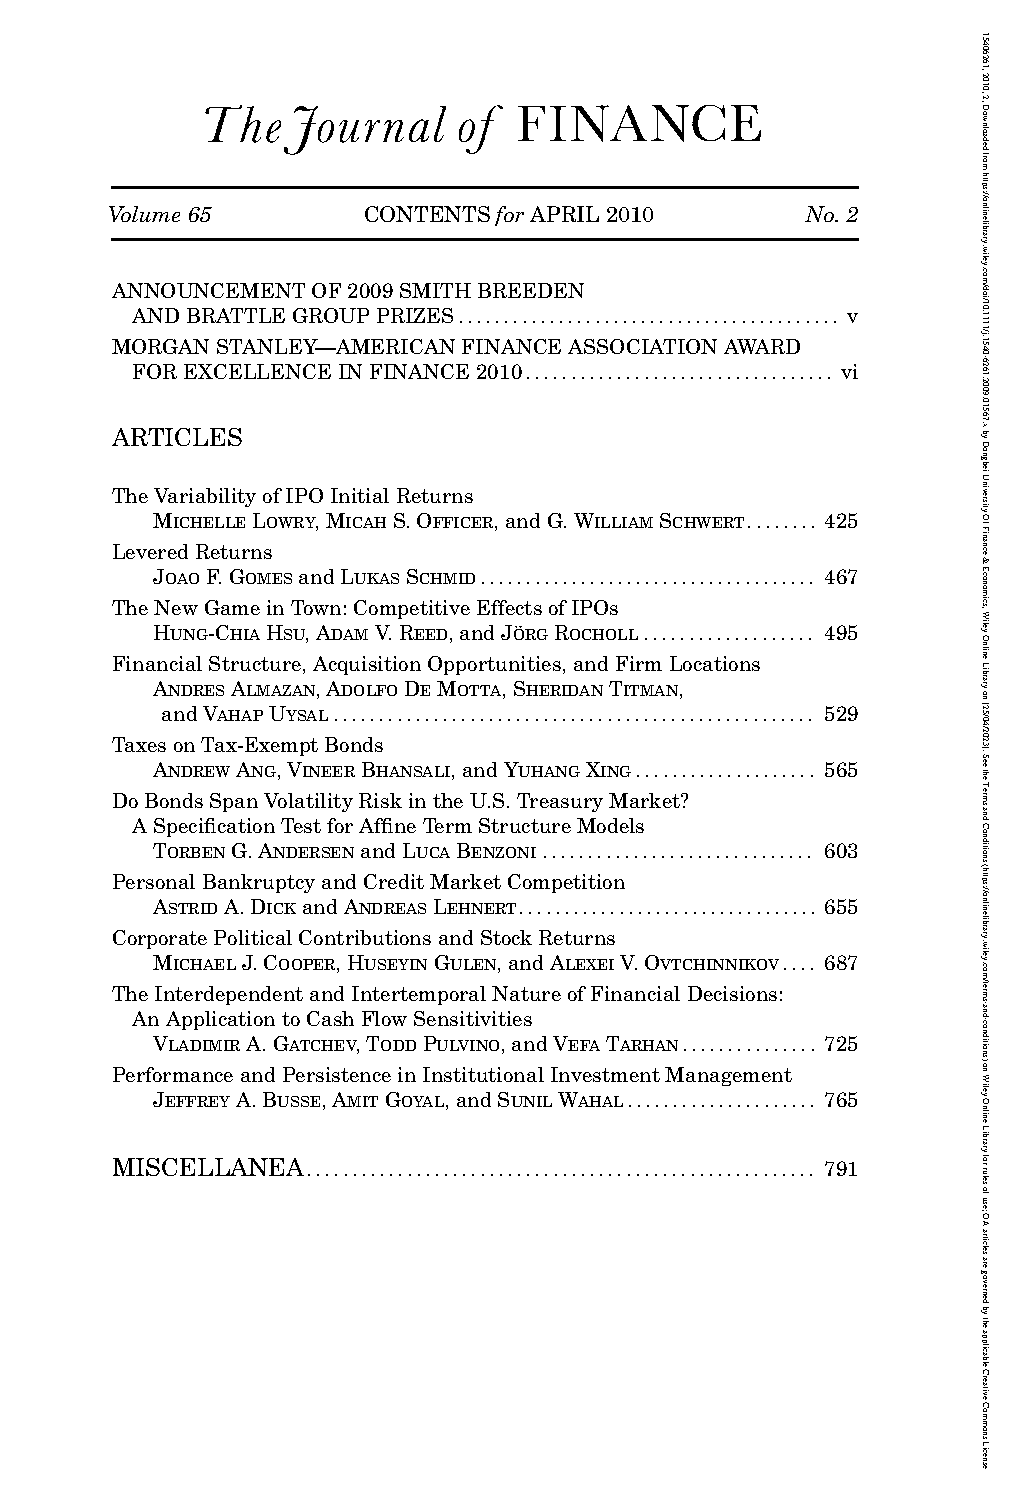
\includegraphics[height=0.7\textheight]{Files/Front}
	\end{figure}
	\begin{center}
		\footnotesize \textit{Hou, Mo, Xue, Zhang.\ \textbf{The Investment CAPM}（剑桥大学出版社，2025）。}
	\end{center}
\end{frame}

\begin{frame}{$q$ 阵营对异象的战绩}
	\begin{figure}
		\centering
		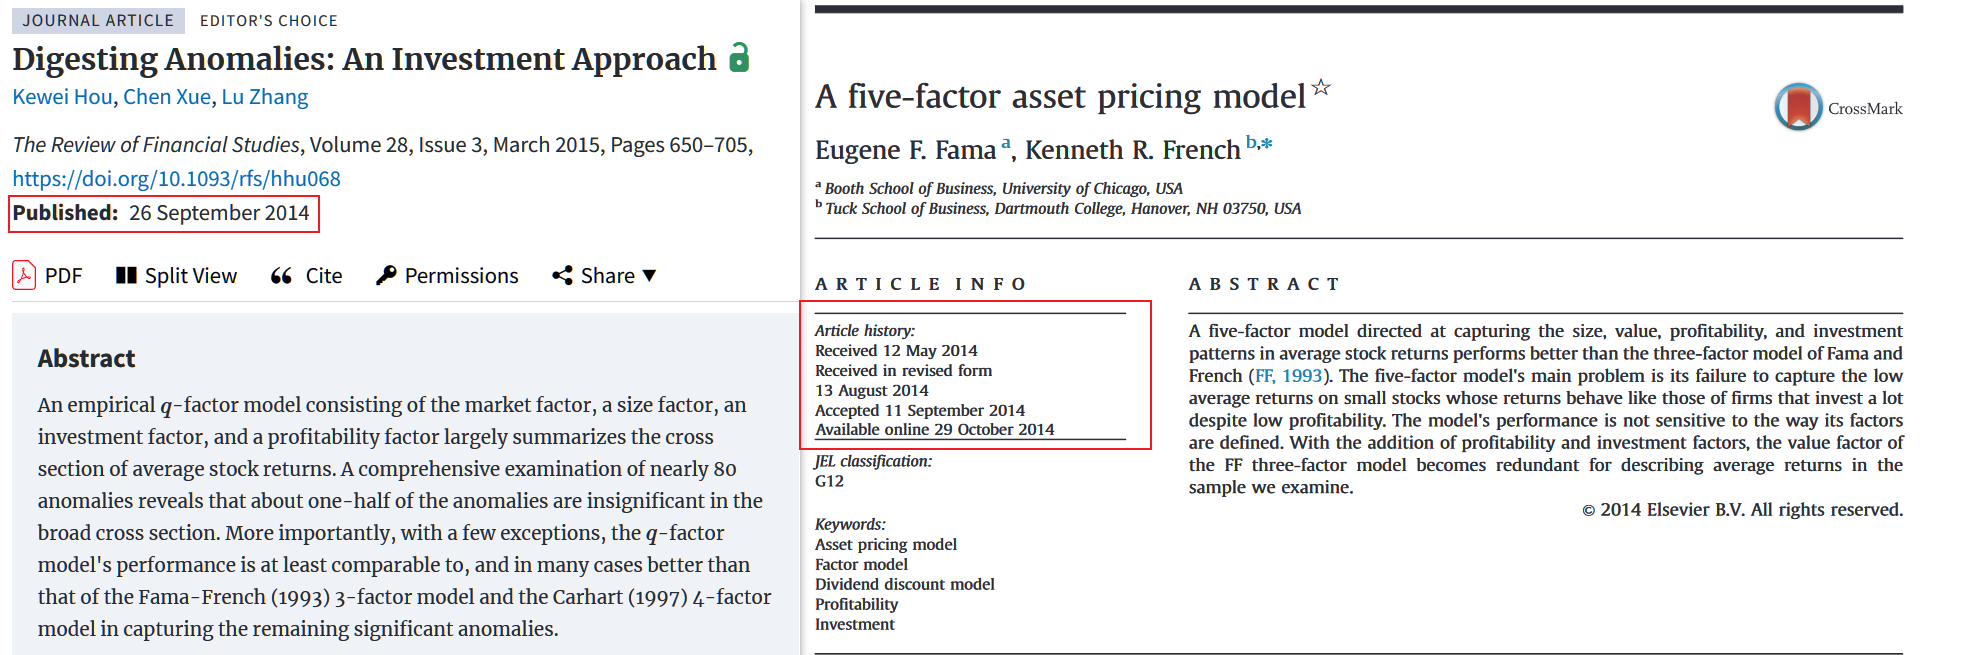
\includegraphics[width=1.0\linewidth]{Files/pk.png}
	\end{figure}
\end{frame}

\end{document}
